\documentclass[tikz, border=2mm]{standalone}

\usepackage{amsmath}
\usepackage[scaled]{helvet}
\usepackage{sansmath}
\renewcommand{\familydefault}{\sfdefault}
\usepackage{pgfplots}
\usepackage{tikz}
\pgfplotsset{compat=1.18}

\usetikzlibrary{arrows.meta, backgrounds, calc, fit, positioning, matrix, shapes.misc}

% ---- Layout constants and colors (auto-generated, edit config.py) ----
% Auto-generated by scripts/03_compile_figure.py — do not edit by hand.
% Edit config.py:ATOMIC_LAYOUT and re-run make.
\def\CanvasW{31.70}
\def\CanvasH{17.50}
\def\FigureTitleX{0.60}
\def\FigureTitleY{0.70}
\def\PanelsY{2.00}
\def\PanelW{9.00}
\def\PanelAW{10.20}
\def\PanelCW{10.20}
\def\PanelH{14.50}
\def\PanelAx{0.60}
\def\PanelBx{11.40}
\def\PanelCx{21.00}
\def\PanelPadX{0.35}
\def\PanelPadY{1.40}
\def\PanelHeaderX{0.20}
\def\PanelHeaderY{0.25}
\def\PanelSubtitleX{0.55}
\def\PanelSubtitleY{0.60}
\def\CardInnerSep{0.20}
\def\PanelAContentW{9.50cm}
\def\PanelAContentInnerW{9.10cm}
\def\PanelBContentW{8.30cm}
\def\PanelBContentInnerW{7.90cm}
\def\PanelCContentW{9.50cm}
\def\PanelCContentInnerW{9.10cm}
\def\PanelContentW{8.30cm}
\def\PanelContentInnerW{7.90cm}
\def\CardGap{0.35}
\def\PanelBObjH{4.50cm}
\def\PanelCCombinedH{6.25cm}
\def\PanelCHypH{6.25cm}
\def\PanelCOutH{3.20cm}
\def\PanelAReqY{3.25}
\def\PanelAOptY{11.60}
\def\PanelBFeatsY{1.75}
\def\PanelBObjY{5.30}
\def\PanelBOptY{10.15}
\def\PanelCValY{3.05}
\def\PanelCCombinedY{3.05}
\def\PanelCOutY{9.65}
\def\PanelAColLeftX{2.25}
\def\PanelAColRightX{7.95}
\def\PanelBColLeftX{2.43}
\def\PanelBColMidX{4.50}
\def\PanelBColRightX{6.58}
\def\PanelCColLeftX{2.25}
\def\PanelCColMidX{5.10}
\def\PanelCColRightX{7.95}
\def\PanelBColLeftXRel{2.08}
\def\PanelBColMidXRel{4.15}
\def\PanelBColRightXRel{6.23}
\def\PanelCColLeftXRel{1.90}
\def\PanelCColMidXRel{4.75}
\def\PanelCColRightXRel{7.60}
\def\FlowLaneY{16.70}
\def\InterPanelChevronY{9.25}
\def\InterPanelChevronSize{15}

% Auto-generated by scripts/03_compile_figure.py — do not edit by hand.
% Edit config.py:COLORS / TIKZ_COLOR_MAP and re-run make.
\definecolor{cTeal}{RGB}{31,157,138}
\definecolor{cLilac}{RGB}{204,204,255}
\definecolor{cCoral}{RGB}{210,100,63}
\definecolor{cGold}{RGB}{210,100,63}
\definecolor{cGoldBright}{RGB}{210,100,63}
\definecolor{cSlate}{RGB}{107,114,128}
\definecolor{cSlateLight}{RGB}{144,164,174}
\definecolor{cNavy}{RGB}{17,24,39}
\definecolor{cGreyMid}{RGB}{107,107,107}
\definecolor{cCharcoal}{RGB}{199,205,212}
\definecolor{cLavender}{RGB}{59,91,165}
\definecolor{cZoneA}{RGB}{248,250,252}
\definecolor{cZoneB}{RGB}{248,250,252}
\definecolor{cZoneC}{RGB}{248,250,252}
\definecolor{cTealLight}{RGB}{232,246,243}
\definecolor{cCoralLight}{RGB}{251,237,231}
\definecolor{cLavenderLight}{RGB}{238,242,251}
\definecolor{cCream}{RGB}{248,250,252}

% --- Color utility macros (auto-generated) ---
\newcommand{\TealText}{\color{cTeal}}
\newcommand{\TealBg}{\colorbox{cTeal}}
\newcommand{\LilacText}{\color{cLilac}}
\newcommand{\LilacBg}{\colorbox{cLilac}}
\newcommand{\CoralText}{\color{cCoral}}
\newcommand{\CoralBg}{\colorbox{cCoral}}
\newcommand{\GoldText}{\color{cGold}}
\newcommand{\GoldBg}{\colorbox{cGold}}
\newcommand{\GoldbrightText}{\color{cGoldBright}}
\newcommand{\GoldbrightBg}{\colorbox{cGoldBright}}
\newcommand{\SlateText}{\color{cSlate}}
\newcommand{\SlateBg}{\colorbox{cSlate}}
\newcommand{\SlatelightText}{\color{cSlateLight}}
\newcommand{\SlatelightBg}{\colorbox{cSlateLight}}
\newcommand{\NavyText}{\color{cNavy}}
\newcommand{\NavyBg}{\colorbox{cNavy}}
\newcommand{\GreymidText}{\color{cGreyMid}}
\newcommand{\GreymidBg}{\colorbox{cGreyMid}}
\newcommand{\CharcoalText}{\color{cCharcoal}}
\newcommand{\CharcoalBg}{\colorbox{cCharcoal}}
\newcommand{\LavenderText}{\color{cLavender}}
\newcommand{\LavenderBg}{\colorbox{cLavender}}
\newcommand{\ZoneaText}{\color{cZoneA}}
\newcommand{\ZoneaBg}{\colorbox{cZoneA}}
\newcommand{\ZonebText}{\color{cZoneB}}
\newcommand{\ZonebBg}{\colorbox{cZoneB}}
\newcommand{\ZonecText}{\color{cZoneC}}
\newcommand{\ZonecBg}{\colorbox{cZoneC}}
\newcommand{\TeallightText}{\color{cTealLight}}
\newcommand{\TeallightBg}{\colorbox{cTealLight}}
\newcommand{\CorallightText}{\color{cCoralLight}}
\newcommand{\CorallightBg}{\colorbox{cCoralLight}}
\newcommand{\LavenderlightText}{\color{cLavenderLight}}
\newcommand{\LavenderlightBg}{\colorbox{cLavenderLight}}
\newcommand{\CreamText}{\color{cCream}}
\newcommand{\CreamBg}{\colorbox{cCream}}


% Declare layers for proper z-ordering
\pgfdeclarelayer{canvas}
\pgfdeclarelayer{background}
\pgfdeclarelayer{midground}
\pgfsetlayers{canvas,background,midground,main}

% Typography commands for inline use
\newcommand{\mathvar}[1]{\text{\fontsize{10}{12}\selectfont\itshape\sffamily\color{cNavy}#1}}

% Safe asset include helper
\newcommand{\safeincludegraphics}[2][]{%
  \IfFileExists{#2}{\includegraphics[#1]{#2}}{\fbox{\scriptsize missing}}%
}

% --- Core Styles ---
\tikzset{panel/.style={rounded corners=12pt, draw=cCharcoal, line width=0.8pt, inner sep=0pt}}
\tikzset{panelA/.style={panel, fill=cZoneA}}
\tikzset{panelB/.style={panel, fill=cZoneB}}
\tikzset{panelC/.style={panel, fill=cZoneC}}

\tikzset{card/.style={rounded corners=8pt, draw=cCharcoal, line width=0.6pt, fill=white, inner sep=\CardInnerSep cm}}
\tikzset{whiteCard/.style={card}}
\tikzset{tealStep/.style={rounded corners=6pt, draw=cCharcoal, line width=0.8pt, fill=white, inner sep=\CardInnerSep cm}}
\tikzset{goldObjective/.style={rounded corners=8pt, draw=cCharcoal, line width=1.0pt, fill=white, inner sep=\CardInnerSep cm}}
\tikzset{coralOptimise/.style={rounded corners=8pt, draw=cCharcoal, line width=1.0pt, fill=white, inner sep=\CardInnerSep cm}}
\tikzset{dashedBox/.style={rounded corners=6pt, draw=cCharcoal, line width=0.8pt, dashed, dash pattern=on 3pt off 2pt, inner sep=\CardInnerSep cm}}

\tikzset{pill/.style={rounded rectangle, draw=cCharcoal, line width=0.8pt, fill=cTealLight, inner sep=3pt, font=\fontsize{8}{9}\selectfont\bfseries\sffamily\color{cNavy}}}
\tikzset{goldpill/.style={rounded rectangle, draw=cCharcoal, line width=0.8pt, fill=cCoralLight, inner sep=2pt, font=\fontsize{8}{10}\selectfont\bfseries\sffamily\color{cNavy}}}
\tikzset{goldborder/.style={rounded corners=8pt, draw=cLavender, line width=1.0pt, fill=cLavenderLight!60, inner sep=4pt}}

% --- Spec-compliant aliases ---
\tikzset{stepbox/.style={card}}
\tikzset{tealbox/.style={tealStep}}
\tikzset{optbox/.style={dashedBox}}
\tikzset{goldbox/.style={goldObjective}}
\tikzset{coralbox/.style={coralOptimise}}

% --- Arrows ---
\tikzset{procArrow/.style={-{Latex[length=4pt]}, thin, color=cSlateLight}}
\tikzset{dashedArrow/.style={-{Latex[length=4pt]}, dashed, dash pattern=on 3pt off 2pt, color=cGreyMid}}
\tikzset{flow_arrow/.style={procArrow, line width=0.8pt}}

% --- Typography ---
\tikzset{figuretitle/.style={font=\fontsize{20}{22}\selectfont\bfseries\sffamily\color{cNavy}}}
\tikzset{panelLabel/.style={font=\fontsize{14}{16}\selectfont\bfseries\sffamily\color{cNavy}}}
\tikzset{panelHeader/.style={font=\fontsize{14}{16}\selectfont\bfseries\sffamily\color{cNavy}}}
\tikzset{panelSubtitle/.style={font=\fontsize{10}{12}\selectfont\sffamily\color{cNavy}}}
\tikzset{cardHeader/.style={font=\fontsize{10}{12}\selectfont\bfseries\sffamily\color{cNavy}}}
\tikzset{moduleTitle/.style={font=\fontsize{10}{12}\selectfont\bfseries\sffamily\color{cNavy}}}
\tikzset{annotation/.style={font=\fontsize{8}{9}\selectfont\itshape\sffamily\color{cGreyMid}}}
\tikzset{labelTeal/.style={font=\fontsize{10}{12}\selectfont\bfseries\sffamily\color{cTeal}}}
\tikzset{labelCoral/.style={font=\fontsize{10}{12}\selectfont\bfseries\sffamily\color{cCoral}}}

% Helper for filled chevrons
\newcommand{\filledchevron}[1]{
  \fill[cNavy] ([xshift=-0.20cm, yshift=-0.35cm]#1) -- ++(0.3,0.35) -- ++(-0.3,0.35) -- ++(0.4,0) -- ++(0.3,-0.35) -- ++(-0.3,-0.35) -- cycle;
}

% Native funnel+gear icon (drawn in-panel to avoid imported-PDF bbox clipping).
% Usage: \funnelgearicon[<scale>] inside a tikzpicture/scope.
\newcommand{\funnelgearicon}[1][1]{%
  \begin{scope}[xscale=#1, yscale=-#1, line join=round, line cap=round]
    % Funnel silhouette and interior channel
    \filldraw[fill=cLilac!36, draw=cLilac, line width=0.42pt]
      (-0.45,-0.50) -- (0.45,-0.50) -- (0.18,-0.15) -- (-0.18,-0.15) -- cycle;
    \fill[white, opacity=0.42]
      (-0.35,-0.45) -- (0.35,-0.45) -- (0.12,-0.21) -- (-0.12,-0.21) -- cycle;
    \draw[cLilac!95!cNavy, line width=0.42pt, opacity=0.85] (-0.45,-0.50) -- (0.45,-0.50);
    \filldraw[fill=cLilac!23, draw=cLilac, line width=0.38pt]
      (-0.08,-0.15) -- (0.08,-0.15) -- (0.06,0.13) -- (-0.06,0.13) -- cycle;

    % Particles flowing through the funnel
    \foreach \px/\py in {
      -0.36/-0.40, -0.21/-0.43, -0.04/-0.41, 0.15/-0.39, 0.33/-0.36,
      -0.28/-0.30, -0.10/-0.33, 0.08/-0.30, 0.25/-0.28,
      -0.03/-0.23, 0.02/-0.19
    }{
      \fill[cNavy, opacity=0.58] (\px,\py) circle[radius=0.015];
    }

    % Gear
    \def\gearcx{0.19}
    \def\gearcy{-0.15}
    \def\gearouter{0.17}
    \def\gearinner{0.08}
    \foreach \ang in {0,45,...,315}{
      \begin{scope}[shift={(\gearcx,\gearcy)}, rotate=\ang]
        \fill[cNavy] (\gearouter,-0.028) rectangle ++(0.052,0.056);
      \end{scope}
    }
    \fill[cNavy, opacity=0.95] (\gearcx,\gearcy) circle[radius=\gearouter];
    \fill[white] (\gearcx,\gearcy) circle[radius=\gearinner];
  \end{scope}%
}

% Auto-generated by scripts/03_compile_figure.py
\def\ProcessedDir{../outputs/processed}
\def\ComponentsSvgDir{../outputs/components/svg}
\def\ComponentsPdfDir{../outputs/components/pdf}
\def\FigureOutDir{../outputs/figure}


\begin{document}
\begin{tikzpicture}[x=1cm, y=-1cm]
\sansmath

\begin{pgfonlayer}{canvas}
\fill[white] (0,0) rectangle (\CanvasW, \CanvasH);
\end{pgfonlayer}

\node[figuretitle, anchor=north west, align=left] at (\FigureTitleX,\FigureTitleY) {
    jaxENT workflow for ensemble-experiment integration and hypothesis testing
};

% ============================================================
% Panel A — Inputs
% ============================================================
\coordinate (pa_nw) at (\PanelAx, \PanelsY);

\begin{pgfonlayer}{background}
\node[panelA, minimum width=\PanelAW cm, minimum height=\PanelH cm, anchor=north west] (panel_A) at (pa_nw) {};
\end{pgfonlayer}

\node[panelLabel, anchor=north west] (a_label) at ($(panel_A.north west) + (\PanelHeaderX, \PanelHeaderY)$) {(a)};

% --- Header Section (Centered) ---
\node[annotation, anchor=north] (a_sub) at ($(panel_A.north) + (0, \PanelSubtitleY)$) {
    \fontsize{10}{12}\selectfont Integration as a statistical connector
};

% --- Required Inputs Container ---
\begin{pgfonlayer}{midground}
\node[whiteCard, minimum width=\PanelAContentW, minimum height=8.0cm, anchor=north] 
    (a_req_box) at ($(panel_A.north west) + (0.5*\PanelAW, \PanelAReqY)$) {};
\end{pgfonlayer}

% Position header relative to box
\node[cardHeader, anchor=north, align=center, text width=\PanelAContentInnerW] (a_req_head) at ($(panel_A.north west) + (0.5*\PanelAW, \PanelAReqY + 0.15)$) {Required inputs};

% Slot coordinates — moved up to give room for bar below
\coordinate (a_col_c) at ($(panel_A.north west) + (\PanelAColLeftX, \PanelAReqY + 1.4)$);
\coordinate (a_col_t) at ($(panel_A.north west) + (\PanelAColRightX, \PanelAReqY + 1.4)$);

% --- Candidate Column (Left) ---
\node[labelTeal, anchor=north] (a_c_tit) at (a_col_c) {Candidate};

% Define consistent Y coordinates for row alignment
\coordinate (a_img_y) at ($(a_c_tit.south) + (0, 1.05)$);
\coordinate (a_text_y) at ($(a_c_tit.south) + (0, 2.0)$);

% Stacked ensembles (centered on column)
\node[anchor=center, opacity=0.2] (a_e_b) at (a_col_c |- a_img_y) {\safeincludegraphics[width=1.8cm]{\ProcessedDir/ensemble_stack.png}};
\node[anchor=center, opacity=0.4] (a_e_m) at (a_e_b.center) {\safeincludegraphics[width=1.8cm]{\ProcessedDir/ensemble_stack.png}};
\node[anchor=center] (a_e_i) at (a_col_c |- a_img_y) {
    \safeincludegraphics[width=2.6cm]{\ProcessedDir/ensemble_stack.png}
};

\node[anchor=north, align=center, text width=4.2cm, scale=0.8, transform shape] (a_s_e) at (a_col_c |- a_text_y) {
    \textbf{Structural Ensembles}\\[0.5mm]
    {\fontsize{8}{9}\selectfont\itshape\sffamily\color{cGreyMid}(From simulations)}\\[1.5mm]
    {\color{cGreyMid}\fontsize{8}{9.5}\selectfont\sffamily
    Molecular Dynamics\\[0.8mm]
    \textit{or}\\[0.8mm]
    AlphaFold2 +\\[0.8mm]
    MSA subsampling\par}
};

% --- Target Column (Right) ---
\node[labelCoral, anchor=north] (a_t_tit) at (a_col_t) {Target};

\node[anchor=center] (a_h_p) at (a_col_t |- a_img_y) {
    \safeincludegraphics[width=2.6cm]{\ComponentsPdfDir/hdx_curves.pdf}
};

\node[anchor=north, align=center, text width=4.2cm, scale=0.8, transform shape] (a_e_d) at (a_col_t |- a_text_y) {
    \textbf{Biophysical Data}\\[0.5mm]
    {\fontsize{8}{9}\selectfont\itshape\sffamily\color{cGreyMid}(From experiments)}\\[1.5mm]
    {\color{cGreyMid}\fontsize{8}{9.5}\selectfont\sffamily
    HDX-MS Uptake Curves\\[0.8mm]
    NMR Protection Factors\\[0.8mm]
    \textit{or}\\[0.8mm]
    SAXS Curves\par}
};

% --- Connector Step (Center) ---
\node[tealStep, anchor=center, align=center, text depth=1mm, inner xsep=6pt, inner ysep=6pt,
      scale=0.8, transform shape] (a_f_m) at (a_req_box.north |- a_img_y) {
    \textbf{Forward model}\\[1mm]
    $\text{f} (x; \beta) \rightarrow Y_{pred} $\\[1mm]
    {\fontsize{7}{8}\selectfont\color{cGreyMid}(Best-Vendruscolo)}
};

% --- Timescale track (bottom of A1) ---
\node[draw=cCharcoal, rounded corners=6pt, line width=0.5pt, 
      minimum width=8.2cm, minimum height=0.55cm, 
      left color=cTeal, right color=cCoral, 
      anchor=south] (a_timescale) at ($(a_req_box.south) - (0, 0.6)$) {};

\node[anchor=west, font=\sffamily\bfseries\color{white}, scale=0.7, xshift=0.5cm] at (a_timescale.west) {Candidate (fs--ms)};
\node[anchor=east, font=\sffamily\bfseries\color{white}, scale=0.7, xshift=-0.5cm] at (a_timescale.east) {Target (ms--days)};

% --- Optional: orthogonal data box (bottom) ---
\begin{pgfonlayer}{midground}
\node[dashedBox, anchor=north, text width=\PanelAContentW - 0.8cm, align=center] 
    (a_opt_box) at ($(panel_A.north west) + (0.5*\PanelAW, \PanelAOptY)$) {
        \textbf{Optional}: orthogonal data for cross-validation
    };
\end{pgfonlayer}

\draw[procArrow] (a_e_i.east) -- (a_f_m.west);
\draw[procArrow] (a_f_m.east) -- (a_h_p.west);

\coordinate (a_optional_anchor_out) at (a_opt_box.south);

% ============================================================
% Panel B — Engine
% Strategy: place each card box first (chained from prev.south),
%            then anchor all content to that box.
% ============================================================
\coordinate (pb_nw) at (\PanelBx, \PanelsY);

\begin{pgfonlayer}{background}
\node[panelB, minimum width=\PanelW cm, minimum height=\PanelH cm, anchor=north west] (panel_B) at (pb_nw) {};
\end{pgfonlayer}

\node[panelLabel, anchor=north west] (b_label) at ($(panel_B.north west) + (\PanelHeaderX, \PanelHeaderY)$) {(b)};
\node[annotation, anchor=north] (b_sub) at ($(panel_B.north) + (0, \PanelSubtitleY)$) {%
    \fontsize{10}{12}\selectfont\color{cGreyMid}Build \& Fit Model};

% ── Card 1: Map Structures to Observables ──────────────────────────────────
\begin{pgfonlayer}{midground}
\node[tealStep, minimum width=\PanelContentW, minimum height=3.2cm, anchor=north] (b_s1_box)
    at ($(panel_B.north west) + (0.5*\PanelW, \PanelBFeatsY)$) {};
\end{pgfonlayer}

\node[cardHeader, anchor=north, align=center, text width=\PanelContentInnerW] (b_s1_h)
    at ($(b_s1_box.north) + (0, 0.15)$) {Map Structures to Observables};

\node[anchor=center] (b_hmap_container)
    at ($(b_s1_box.north west) + (\PanelBColLeftXRel, 1.85)$) {
    \begin{tikzpicture}[baseline={(b_h.center)}]
        \node[opacity=0.45, xshift=2pt, yshift=2pt] (b_h_bg) {\safeincludegraphics[width=1.3cm]{\ComponentsPdfDir/heatmap_thumb.pdf}};
        \node (b_h) {\safeincludegraphics[width=1.3cm]{\ComponentsPdfDir/heatmap_thumb.pdf}};
        \node[annotation, rotate=90, anchor=south, inner sep=3pt] at (b_h.west) {\fontsize{6.5}{7.5}\selectfont residues};
        \node[annotation, anchor=north, inner sep=2pt] at (b_h.south) {\fontsize{6.5}{7.5}\selectfont frames};
        \node[annotation, anchor=south, scale=0.9, yshift=2pt] at (b_h.north) {(x H-bonds, contacts, ... )};
    \end{tikzpicture}
};

\node[anchor=center] (b_arrow)
    at ($(b_s1_box.north west) + (\PanelBColMidXRel, 1.85)$) {
    \tikz \draw[procArrow, line width=0.8pt] (0,0) -- (0.8,0);
};

\node[anchor=center] (b_r_p)
    at ($(b_s1_box.north west) + (\PanelBColRightXRel, 1.85)$) {
    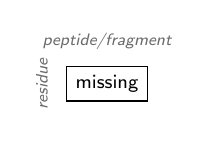
\begin{tikzpicture}[baseline={(b_rp.center)}]
        \node (b_rp) {\safeincludegraphics[width=2.0cm]{\ComponentsPdfDir/residue_peptide.pdf}};
        \node[annotation, rotate=90, anchor=south, inner sep=3pt] at (b_rp.west) {\fontsize{6.5}{7.5}\selectfont residue};
        \node[annotation, anchor=south, inner sep=2pt] at (b_rp.north) {\fontsize{6.5}{7.5}\selectfont peptide/fragment};
    \end{tikzpicture}
};

% ── Card 2: Define Objective ───────────────────────────────────────────────
\begin{pgfonlayer}{midground}
\node[goldObjective, minimum width=\PanelContentW, minimum height=\PanelBObjH, anchor=north] (b_s3_box)
    at ($(b_s1_box.south) + (0, \CardGap)$) {};
\end{pgfonlayer}

\node[cardHeader, anchor=north, align=center, text width=\PanelContentInnerW] (b_s3_h)
    at ($(b_s3_box.north) + (0, 0.15)$) {Define Objective};

\node[anchor=north, align=center, scale=0.8, transform shape] (b_loss_eq)
    at ($(b_s3_h.south) + (0, 0.50)$) {
    \color{cCoral}\rmfamily
    {\fontsize{26}{30}\selectfont $\mathcal{L}$} 
    \raisebox{0.6ex}{\fontsize{12}{17}\selectfont = Data Fidelity + Plausibility + Priors}
};

\node[whiteCard, scale=0.8, transform shape, anchor=center, align=center,
      text width=2.6cm, minimum width=3.0cm, minimum height=1.5cm, inner sep=0pt]
    (b_v_l) at ($(b_s3_box.north west) + (\PanelBColLeftXRel, 3.1)$)
    {\textbf{Error + Work}\\ {\fontsize{7}{8}\selectfont\color{cGreyMid}(Maximum Entropy)}};

\node[anchor=center] (b_gear)
    at ($(b_s3_box.north west) + (\PanelBColMidXRel, 3.1)$) {%
    
\begin{tikzpicture}[x=1cm, y=1cm, baseline=(current bounding box.center)]
        \funnelgearicon[1.5]
    \end{tikzpicture}%
};

\node[whiteCard, scale=0.8, transform shape, anchor=center, align=center,
      text width=2.6cm, minimum width=3.0cm, minimum height=1.5cm, inner sep=0pt]
    (b_v_r) at ($(b_s3_box.north west) + (\PanelBColRightXRel, 3.1)$)
    {\textbf{+ Knowledge}\\ {\fontsize{7}{8}\selectfont\color{cGreyMid}(e.g. covariance)}};

% ── Card 3: Fit to Target ──────────────────────────────────────────────────
\begin{pgfonlayer}{midground}
\node[coralOptimise, minimum width=\PanelContentW, minimum height=3.2cm, anchor=north] (b_s4_box)
    at ($(b_s3_box.south) + (0, \CardGap)$) {};
\end{pgfonlayer}

\node[cardHeader, anchor=north, align=center, text width=\PanelContentInnerW] (b_s4_h)
    at ($(b_s4_box.north) + (0, 0.15)$) {Fit to Target};

\node[anchor=north, align=center] (b_params_box) at ($(b_s4_h.south) + (0, 0.15)$) {
    \fontsize{9}{11}\selectfont
    \renewcommand{\arraystretch}{0.9}
    \begin{tabular}{c@{\hspace{6pt}}l @{\hspace{1.0cm}} c@{\hspace{6pt}}l}
        \color{cNavy}$\omega$ & & \color{cNavy}$\beta$ & \\[-2pt]
        \safeincludegraphics[width=0.8cm]{\ComponentsPdfDir/tiny_bar_chart.pdf} & \shortstack[l]{\textbf{Relative} \\ \textbf{Populations}} &
        \safeincludegraphics[width=1.0cm]{\ComponentsPdfDir/tiny_sliders.pdf} & \shortstack[l]{\textbf{Forward-Model} \\ \textbf{Parameters}}
    \end{tabular}
};

\node[annotation, anchor=north] (b_si_t) at ($(b_params_box.south) + (0, -0.05)$)
    {Differentiable fitting of both structures and conditions};

\matrix (b4_m) [anchor=south, column sep=0.6cm] at ($(b_s4_box.south) + (0, 0.3)$) {
    \node[pill] {modular}; & \node[pill] {efficient}; & \node[pill] {scalable}; \\
};

\draw[procArrow, line width=1.2pt, color=black] (b_s1_box.south) -- (b_s3_box.north);
\draw[procArrow, line width=1.2pt, color=black] (b_s3_box.south) -- (b_s4_box.north);

% ============================================================
% Panel C — Quantify Robustness
% Strategy: align C's cards with Panel B's boundaries, then tighten.
%           B1 area + B2 area -> Combined C12
%           B3 area -> C3
% ============================================================
\coordinate (pc_nw) at (\PanelCx, \PanelsY);

\begin{pgfonlayer}{background}
\node[panelC, minimum width=\PanelCW cm, minimum height=\PanelH cm, anchor=north west] (panel_C) at (pc_nw) {};
\end{pgfonlayer}

\node[panelLabel, anchor=north west] (c_label) at ($(panel_C.north west) + (\PanelHeaderX, \PanelHeaderY)$) {(c)};
\node[annotation, anchor=north] (c_subtitle_text)
    at ($(panel_C.north) + (0, \PanelSubtitleY)$)
    {\fontsize{10}{12}\selectfont\color{cGreyMid}Quantify Robustness};

% ── Combined Card: Validation and Hypothesis Testing ───────────────────────
% Height reduced for compactness: 7.4cm (was 8.05cm)
\begin{pgfonlayer}{midground}
\node[goldObjective, minimum width=\PanelCContentW, minimum height=6.25cm, anchor=north] (c_combined_box)
    at ($(panel_C.north west) + (0.5*\PanelCW, \PanelCCombinedY)$) {};
\end{pgfonlayer}

\node[cardHeader, anchor=north, align=center, text width=\PanelCContentInnerW] (c12_header)
    at ($(c_combined_box.north) + (0, 0.15)$) {Validation and Hypothesis Testing};

% ── Hypothesis content — upper portion (centred at Y_rel 2.6) ──────────────

\coordinate (c_hyp_list_ctr)
    at ($(c_combined_box.north west) + (\PanelCColLeftXRel, 2.6)$);

\node[anchor=center, scale=0.85] (c_h2_img) at (c_hyp_list_ctr)
    {\safeincludegraphics[width=1.22cm]{\ProcessedDir/h2_coral.png}};
\node[anchor=east, align=center, scale=0.8, xshift=-0.0cm] (c_h2_lbl) at (c_h2_img.west)
    {\fontsize{8}{9}\selectfont\bfseries H$_2$\\\fontsize{7}{8}\selectfont(85\%)};

\node[anchor=south, scale=0.85, yshift=0.18cm] (c_h1_img) at (c_h2_img.north)
    {\safeincludegraphics[width=1.22cm]{\ProcessedDir/h1_teal.png}};
\node[anchor=east, align=center, scale=0.8, xshift=-0.0cm] (c_h1_lbl) at (c_h1_img.west)
    {\fontsize{8}{9}\selectfont\bfseries H$_1$\\\fontsize{7}{8}\selectfont(0\%)};

\node[anchor=north, scale=0.85, yshift=-0.18cm] (c_h3_img) at (c_h2_img.south)
    {\safeincludegraphics[width=1.22cm]{\ProcessedDir/h3_lavender.png}};
\node[anchor=east, align=center, scale=0.8, xshift=-0.0cm] (c_h3_lbl) at (c_h3_img.west)
    {\fontsize{8}{9}\selectfont\bfseries H$_3$\\\fontsize{7}{8}\selectfont(15\%)};

\node[annotation, anchor=north, align=center] (c_hyp_annot)
    at ($(c_h3_img.south) + (0, -0.2)$) {($\omega$ \%)};

% Scorecard (middle column)
\node[anchor=center, scale=0.85] (c_scorecard)
    at ($(c_combined_box.north west) + (\PanelCColMidXRel, 2.6)$)
    {\safeincludegraphics[width=2.45cm]{\ComponentsPdfDir/scorecard.pdf}};

% Best hypothesis (right column)
\node[goldborder, anchor=center, inner sep=0.25cm, scale=0.95] (c_best_hypothesis)
    at ($(c_combined_box.north west) + (\PanelCColRightXRel, 2.6)$)
    {\safeincludegraphics[width=1.60cm]{\ProcessedDir/best_hypothesis.png}};
\node[anchor=north, align=center,
      font=\fontsize{9}{10}\selectfont\bfseries\sffamily\color{cLavender}, yshift=1pt]
    at (c_best_hypothesis.south) {Best\\Hypothesis};

% Arrows
\draw[procArrow] (c_h1_img.east) -- ($(c_scorecard.west) + (0, -0.62)$);
\draw[procArrow] (c_h2_img.east) -- (c_scorecard.west);
\draw[procArrow] (c_h3_img.east) -- ($(c_scorecard.west) + (0, 0.62)$);
\draw[procArrow] (c_scorecard.east) -- (c_best_hypothesis.west);

% ── Validation pills — bottom portion (centred at Y_rel 6.2) ───────────────
% Shifted UP as well to close gap

\node[tealbox, scale=0.8, anchor=center, align=center,
      minimum width=3.0cm, minimum height=1.22cm, text width=2.6cm, inner sep=0pt]
    (c_v1) at ($(c_combined_box.north west) + (\PanelCColLeftXRel, 5.5)$)
    {Split types /\\Replicates};
\node[tealbox, scale=0.8, anchor=center, align=center,
      minimum width=3.0cm, minimum height=1.22cm, text width=2.6cm, inner sep=0pt]
    (c_v2) at ($(c_combined_box.north west) + (\PanelCColMidXRel, 5.5)$)
    {Robust success\\metrics};
\node[optbox, scale=0.8, anchor=center, align=center,
      minimum width=3.0cm, minimum height=1.22cm, text width=2.6cm, inner sep=0pt,
      font=\color{cGreyMid}\sffamily]
    (c_v3) at ($(c_combined_box.north west) + (\PanelCColRightXRel, 5.5)$)
    {Cross-validation\\(orthogonal data)};

% ── Card 3: Outputs (interpretable) ────────────────────────────────────────
% Height 3.2cm. It follows c_combined_box.south, so bringing up the box
% naturally brings up this secondary card to match the cluster.
\begin{pgfonlayer}{midground}
\node[coralOptimise, minimum width=\PanelCContentW, minimum height=3.2cm, anchor=north] (c_outputs_box)
    at ($(c_combined_box.south) + (0, \CardGap)$) {};
\end{pgfonlayer}

\node[cardHeader, anchor=north, align=center, text width=\PanelCContentInnerW] (c3_header)
    at ($(c_outputs_box.north) + (0, 0.15)$) {Outputs (interpretable)};

% Symbol row
\node[anchor=base, color=cNavy, scale=0.8] 
    at ($(c_outputs_box.north west) + (\PanelCColLeftXRel, 1.0)$) {$\omega$};
\node[anchor=base, color=cNavy, scale=0.8] 
    at ($(c_outputs_box.north west) + (\PanelCColMidXRel, 1.0)$) {$\beta, \omega$};

% Images row
\node[anchor=center, scale=0.8] 
    at ($(c_outputs_box.north west) + (\PanelCColLeftXRel, 1.6)$) {\safeincludegraphics[width=1.4cm]{\ComponentsPdfDir/weight_dist.pdf}};
\node[anchor=center, scale=0.8] 
    at ($(c_outputs_box.north west) + (\PanelCColMidXRel, 1.6)$) {\safeincludegraphics[width=1.4cm]{\ComponentsPdfDir/tiny_sliders.pdf}};
\node[anchor=center, scale=0.8] 
    at ($(c_outputs_box.north west) + (\PanelCColRightXRel, 1.6)$) {\safeincludegraphics[width=1.4cm]{\ProcessedDir/residue_work.png}};

% Labels row
\node[annotation, anchor=north, align=center] (c3_thumb_weightdist)
    at ($(c_outputs_box.north west) + (\PanelCColLeftXRel, 2.2)$) {Structural\\ distributions};
\node[annotation, anchor=north, align=center] (c3_thumb_params)
    at ($(c_outputs_box.north west) + (\PanelCColMidXRel, 2.2)$) {Model-level\\ uncertainty};
\node[annotation, anchor=north, align=center] (c3_thumb_struct)
    at ($(c_outputs_box.north west) + (\PanelCColRightXRel, 2.2)$) {Ensemble-level\\ uncertainty};


% ── End of Panel C ────────────────────────────────────────────────────────


% Main inter-panel flow (Chevrons)
\coordinate (chevron_y_ref) at (0,\InterPanelChevronY);
\path (panel_A.east) -- (panel_B.west) coordinate[midway] (ab_mid);
\path (panel_B.east) -- (panel_C.west) coordinate[midway] (bc_mid);

% Robust drawn chevrons instead of pointed arrows
\filledchevron{ab_mid |- chevron_y_ref}
\filledchevron{bc_mid |- chevron_y_ref}

% Optional dashed route in bottom lane
\coordinate (flow_lane_ref) at (0,\FlowLaneY);
\coordinate (opt_lane_right) at (bc_mid |- flow_lane_ref);

% Terminate on weight distribution thumbnail in C
\coordinate (opt_target) at (c3_thumb_weightdist.south);

% Draw behind everything (background layer)
\begin{pgfonlayer}{background}
\end{pgfonlayer}

\draw[dashedArrow, line width=1.2pt, rounded corners=6pt]
  (a_optional_anchor_out.center) -- (a_optional_anchor_out.center |- flow_lane_ref)
  -- (opt_target |- flow_lane_ref)
  -- (opt_target);

\end{tikzpicture}
\end{document}
